\documentclass[11p,a4paper]{article}

\usepackage{amsmath, amssymb,enumerate,arev,xcolor,graphicx, nicefrac}

\title{Board Questions}
\date{Fourth Session, Sep 26th}

\begin{document}
\maketitle

\section{Bernoulli RVs}
\begin{enumerate}
\item Prove: if $ X \sim Bernoulli p $ then $ var(X) = p(1-p) $
\item Prove: if $ X \sim bin(n,p) $ then $ var(X) = np(1-p) $
\item Suppose $ X_{1}, ldots, X_{n} $ are independent and all have the same 
standard deviation $ \sigma = 2 $. Let $ \overline{X} $ be the average of
$ X_{1}, ldots, X_{n} $. What is the standard deviation of $ X $?
\end{enumerate}

\section{Probability Table}
\begin{figure}[ht!]
\center
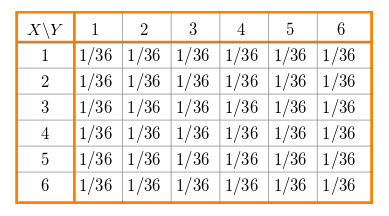
\includegraphics[scale=.6]{table.png} 
\end{figure}
Compute $ F(3.5,4) $.

\section{Computing Covariance}
Flip a fair coin 3 times. Let $ X $ be the number of heads in the first two flips and $ Y $ be
the number of heads in the last two flips. Compute $ Cov(X,Y) $.

\section{Concept Question}
Toss a fair coin $ 2n+1 $ times. Let $ X $ be the number of heads on the first $ n+1 $ trials and 
$ Y $ be the number of heads on the last $ n+1 $ trials.

If $ n=1000 $ then $ Cov(X,Y) $ is 
\begin{enumerate}[a)]
\item 0
\item $ \nicefrac{1}{4} $
\item $ \nicefrac{1}{2} $
\item $ 1 $
\item more than 1
\item tiny but not 0
\end{enumerate}

\end{document}

